\section{Data Center vs. WAN Latency}
\label{sec:latency-DC}

\subsection{Methodology}
Our primary goal in this section is to understand the percentage of total latency (as experienced by end-users) spent inside of the data center (DC). We designed the following experiment to perform queries to data centers. We present the model of communication we expect between end-users and the DC in Fig.\,\ref{fig:DC_model}.

\begin{figure}
  \centering
  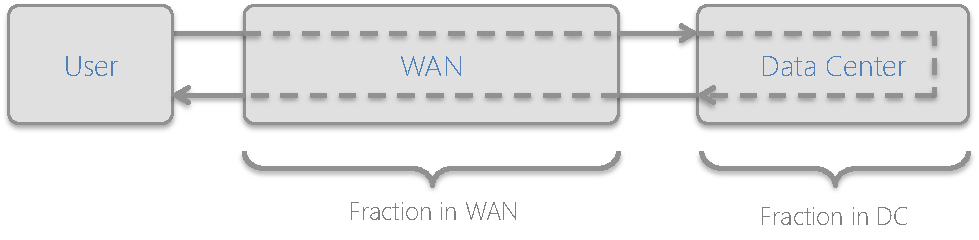
\includegraphics[width=\linewidth]{../figs/DC_model.pdf}
  \vspace{-1em}
  \caption{Typical User-DC communication pattern}
  \label{fig:DC_model}
\end{figure}

We have chosen Google Search as a representative user-facing service for our case study. One reason for choosing Google Search is that the service provides a metric of estimated time spent within the DC (Fig.\,\ref{fig:google_time}). From our analysis in Sec.\,\ref{sec:dc-analysis}, we believe this data to be fairly accurate in reflecting the fraction of time spent inside the DC.

\begin{figure}[t]
  \centering
  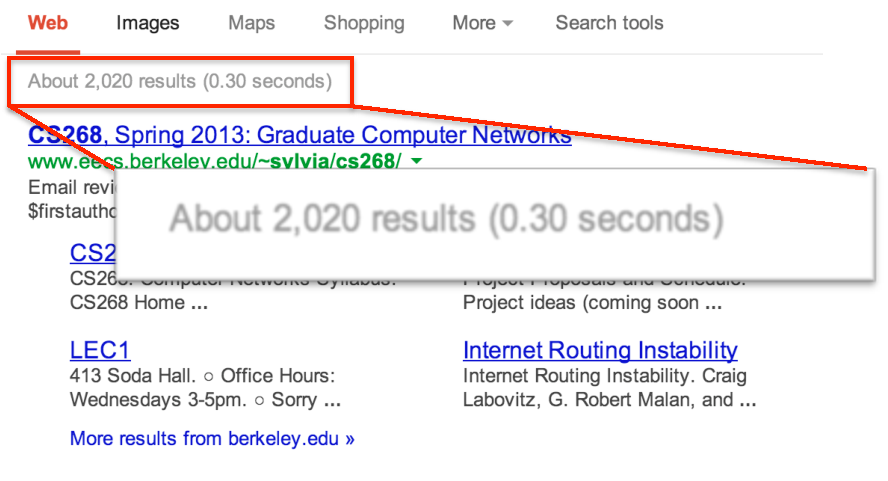
\includegraphics[width=0.85\linewidth]{../figs/GoogleTime.pdf}
  \vspace{-0.7em}
  \caption{Google Search estimated time spent within DC as presented in the search results page}
  \label{fig:google_time}
\end{figure}

We perform a query at the end-host and time-stamp the start and end times. In this way we can measure the complete round-trip time for a single query as experienced by the end-host. The largest hurdle is selecting a search term to query. Initially, we suspected that caching within the DC would impact our results. Thus, we believed that ``hot trends'' (Google's own reported highest searched terms) were likely to be cached. As such, they would provide a baseline measurement for understanding the WAN latency as minimal time spent would be spent within the DC. On the other hand, we use a random string in our queries to minimize the probability of caching and force the query to be processed. We extracted ``hot trends'' from Google Trends\footnote{http://www.google.com/trends/hottrends}, and we generate random strings of length 32, comprised of numbers and letters (both lower and uppercase). Our analysis in Sec.\,\ref{sec:dc-analysis} shows that the results of our measurements differed greatly from our original assumptions. Nonetheless, we believe this methodology is useful in understanding the fraction of round-trip time spent inside the DC.

To provide context for our measurements, we perform \texttt{ICMP ping} queries to measure the network latency from the end-user to Google. Because we conduct this experiment in a geographically distributed fashion and Google has many user-facing servers/IPs, we must take additional steps to ensure the server being pinged is in fact responsible for handing our search queries. We process the application layer HTTP conversation using \texttt{tcpdump} to capture all the packets and extract the IP of the Google server.
 
In Table \ref{tab:DC_method} we provide an overview of the four different ``time'' measurements derived from our experiment. One thing to notice is that Google time is present only when the query returns results. For the 32-character random string, there is no Google time.

\begin{table}
  \begin{tabular}{p{2.3cm} | p{5.5cm}}
    \hline
    type & description \\
    \hline
    Hot-trend-query time & the time spent to query a hot trend word to Google. \\
    \hline
    Random-query time & the time spent to query a 32-character random string.  \\
    \hline
    Ping time & the networking layer round-trip time to the responded Google IP address. \\
    \hline
    Google time & Google's own estimated time spent within their DC. \\
    \hline
  \end{tabular}
  \vspace{1em}
  \caption{Four different ``times'' measured}
  \label{tab:DC_method}
\end{table}


% \begin{itemize}
% \setlength{\leftmargin}{-1pt}
% \setlength{\itemsep}{1pt}
% \setlength{\parskip}{0pt}
% \setlength{\parsep}{0pt}
% \item Hot-trend-query time \\
%   the time spent to query a hot trend word to Google. 
% \item Random-query time -- the time spent to query a 32-character random string. 
% \item Ping time -- the networking layer round-trip time to the responded Google IP address.
% \item Google time -- Google's estimated time spent within their DC.
% \end{itemize}


\subsection{Implementation and Experiment}
\label{sec:impl-exper}

We implemented our measurement script in Python, and use \texttt{cron} to schedule the execution every two hours. In each pass, the script will first visit Google Trends webpage and obtain the hot-trend words for that hour. Along with randomly generated strings, we create a list of 20 strings. The entire list is then queried repeatedly 10 times, and the four ``times'' are recorded. Each query is conducted using Python urllib2 library over HTTP, using the query address \url{http://www.google.com/search?hl=en\&output=search\&q=query}.\footnote{One thing to note about our implementation is that it violates Google's terms of service, as sending automated queries is disallowed. If the automated queries are detected, Google responds with a page containing the following message: ``Our systems have detected unusual traffic from your computer network.'', and the users will be required to enter a CAPTCHA. The workaround we utilize is to limit the query speed. So after each query, we delay the script for 5 seconds. We should point out that there are at most $12\times10\times20$ queries per node per day, which limits our sample size.}

As has been mentioned, while performing a query, we utilize \texttt{tcpdump} to monitor the incoming and outgoing traffic on port 80. By inspecting the TCP traces, we can find the specific Google IP that responds our query. We then \texttt{ping} this IP 10 times and record the results. \texttt{tcpdump} and \texttt{ping} are invoked using Python subprocess module.

We deployed our code on 19 PlanetLab nodes, however, due to crashes, only 13 nodes produced results during the measurement period (Apr.\,18 - Apr.\,25).

\subsection{Analysis}
\label{sec:dc-analysis}

In Fig.\,\ref{fig:data_center}, we show the obtained results from our measurements. On the left, we show the median value of the random query time, hot-trend query time, google time and ping time. On the right, we divide the Google time by hot-trend query time to calculate the portion of time spent inside the DC. The average value for each node is plotted on the right.

First, we noticed that random queries usually take less time than hot-trend queries. This contradicts our initial assumptions about caching. It may be the case that hot-trend queries are not cached by Google's user-facing servers. All queries may be fully processed by the data center. The difference between random query time and hot-trend query time may be accounted for if it is less work because there are no results for a random query. Hot-trends would take a longer time to process because there are associated results.  Despite the fact that many people are searching for hot-trend terms, there is also a high chance some new pages about these words appear. Since Google guarantees relatively fresh search results, having the search continuously processed on every request can provide a better search experience to the public.

Another thing to notice is that though the ping time, and query time vary a lot across these test points, the Google time is relatively stable (around 0.2 seconds). So the Google portion's variation is primarily determined by the WAN performance. For ``6test.edu.cn'' machine in China, each single query takes about 1 second to finish, making the Google portion around 22\%. But generally the time within WAN and DC are fairly close for an end-user, which means that optimization on either side might benefit the user. We ask the questions ``What if WAN latency is minimal, how large of the benefit will be derived from DC improvement?''

\begin{figure*}[!htb]
  \centering
  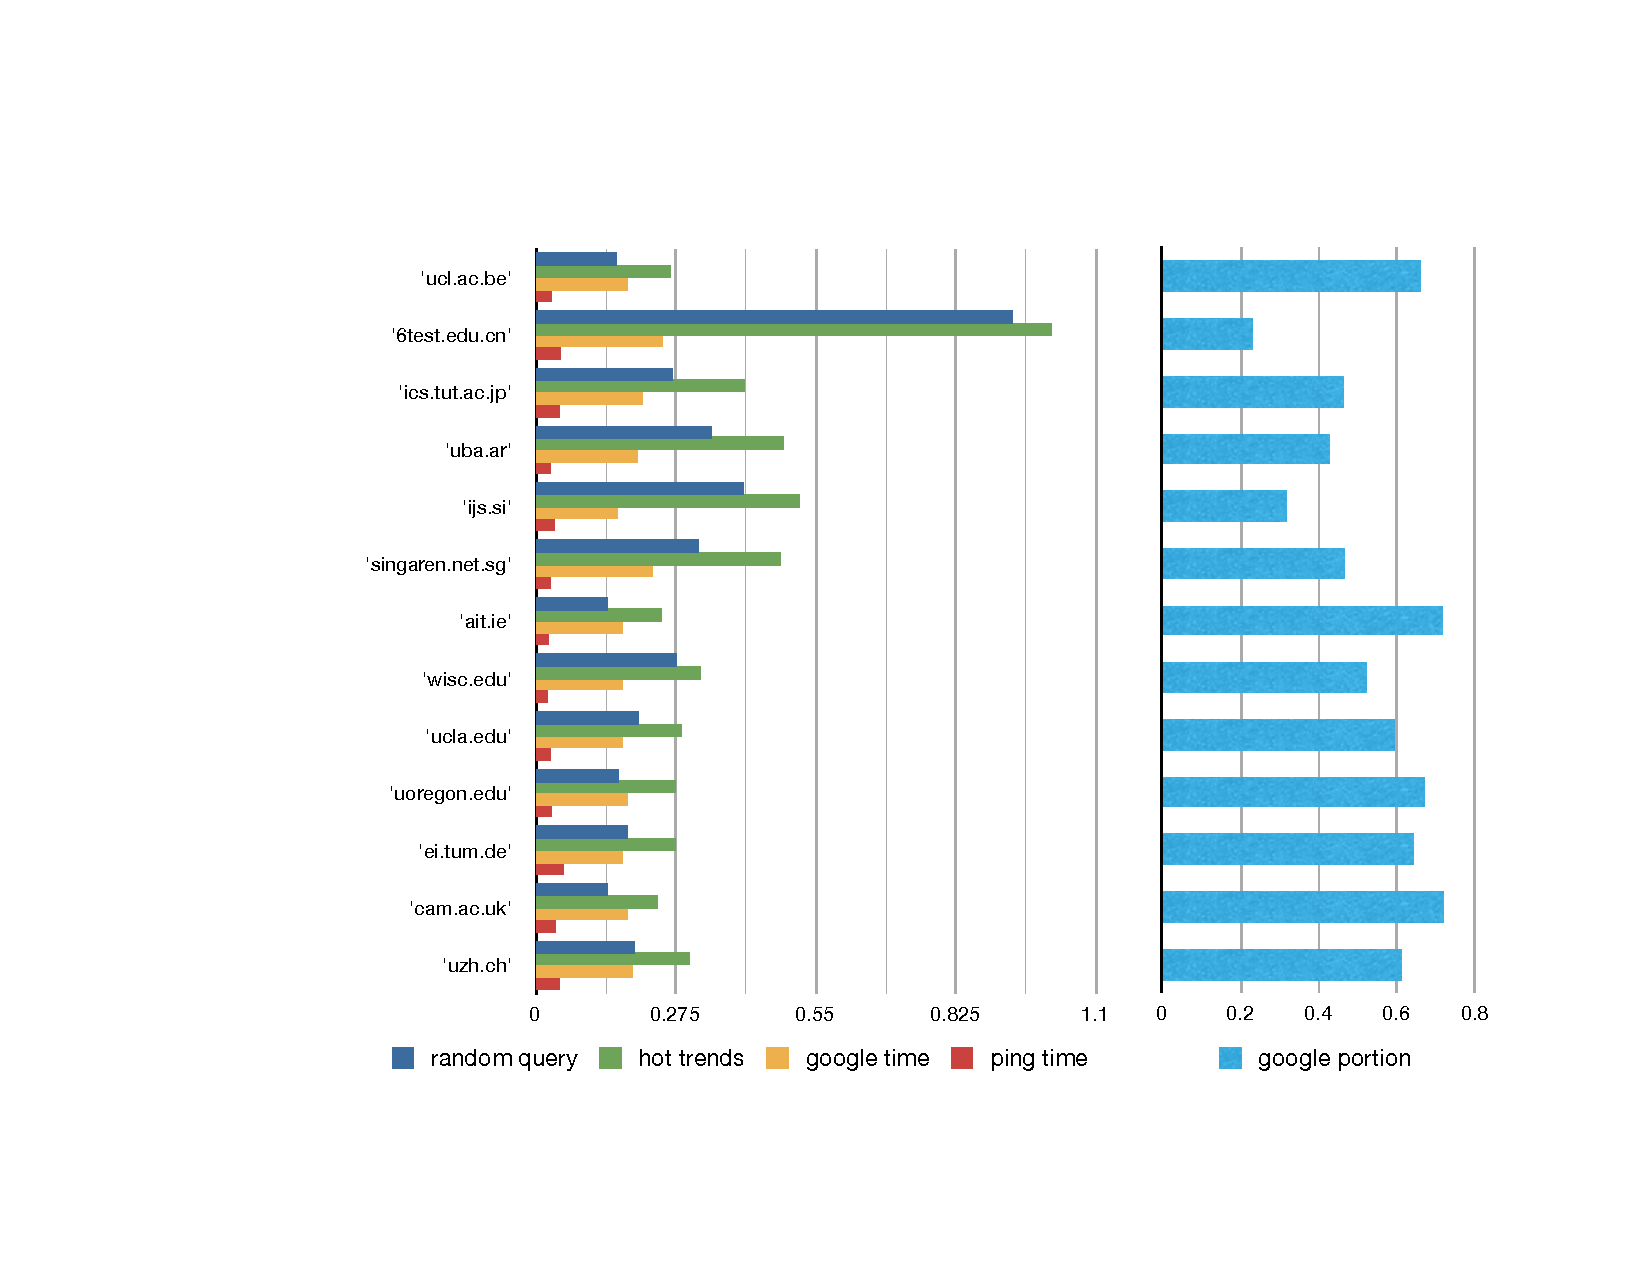
\includegraphics[width=\linewidth]{../figs/data_center.pdf}
  \vspace{-1em}
  \caption{(Left) Four different ``times'' in our DC vs. WAN experiment. (Right) The average of Google time portion within a query conversation for each PlanetLab node test point.}
  \label{fig:data_center}
\end{figure*}

\begin{figure}
  \centering
  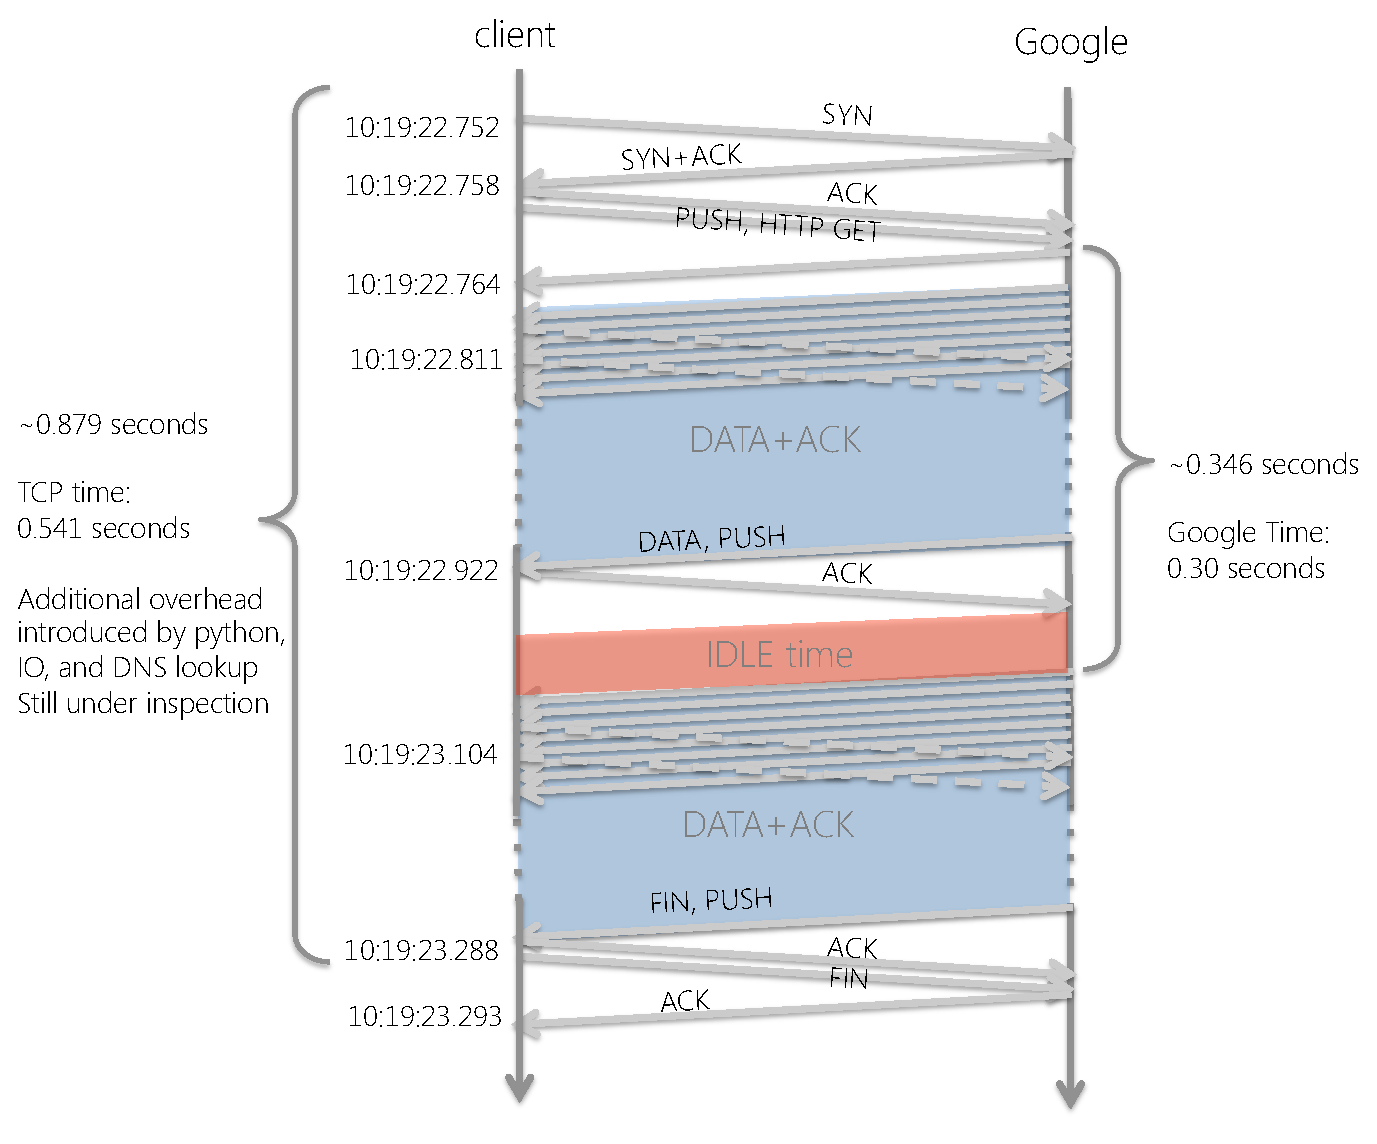
\includegraphics[width=\linewidth]{../figs/tcpdump.pdf}
  \vspace{-1em}
  \caption{One example \texttt{tcpdump} analysis in Google query}
  \label{fig:tcpdump}
\end{figure}

To answer these ``what if'' question, we begin the analysis with an example in \texttt{tcpdump} trace (Fig.\,\ref{fig:tcpdump}). This data was collected in Berkeley EECS-secure wireless network when we searched the term ``CS268''. The \texttt{ping} time to Google is around 5 ms (we believe this is a fairly good connection). In the figure, we've annotated the trace with timestamps, such as ``10:19:22.752'', for illustration. In a typical HTTP (TCP) conversation, after the three-way handshake, the client sends out the query -- HTTP GET, the server then responds with the data. For DC-involved services, there may be a delay since the query has be to processed. However, the server might take another strategy, as observed in Google Search -- it can send out part of the final results first (some javascript, CSS part). Then when the task is finished inside DC, the rest of the results are sent back. Each return page from Google Search is around 200KB, and pipelining them can largely reduce the amount of overall latency experienced by end-users. 

From this graph, one possible argument is that if we optimize the DC performance, reducing the Google Time, what we end up with is reducing the ``idle time'' shown in the figure. It is actually not a large segment of the whole HTTP conversation. And we should point out that this is the case when the average network latency to Google is around 5 ms. For those end-hosts with even poorer network connections, the idle time segment might even be neglectable when there are always data transmission on the fly. Additional experiments are needed to validate this argument, which we leave to future work.

%%% Local Variables: 
%%% mode: latex
%%% TeX-master: "main"
%%% End: 

